\documentclass[17pt, a1paper, portrait]{tikzposter}
\usepackage[utf8]{inputenc}
\usepackage{graphicx}
\usepackage{amsmath}
\graphicspath{{./poster\_images/}}
\usepackage{xcolor}
\usepackage{changepage}
\usepackage{multicol}
\definecolor{eurecomblue}{RGB}{0,159,227}
\definecolor{visuwalkorange}{RGB}{200,160,0}

\tikzposterlatexaffectionproofoff


% RAJOUTER TITRE DU PROJET, AUTEURS
% 30% TEXTE, 40% ILLU, 30% VIDE
% PRECISER CHALLENGE TECHNIQUES
% RESULTATS
% CONCLUSION
% AMELIORATIONS, REFERENCES



\definebackgroundstyle{eurecom}{
\node[inner sep=0pt] at (0,0){
    
\includegraphics[width = \paperwidth,
    height = \paperheight]
    {poster-template.pdf}};
}

\defineblockstyle{bestblockstyle}{
titlewidthscale=0.9, bodywidthscale=1,titleleft,
titleoffsetx=0pt, titleoffsety=0pt, bodyoffsetx=0mm,
bodyverticalshift=10mm, roundedcorners=5,
titleinnersep=5mm, bodyinnersep=4mm,
bodyoffsety=8mm
}
{
\draw[color=eurecomblue, fill=blockbodybgcolor, line width=3pt,
rounded corners=\blockroundedcorners] (blockbody.south west)
rectangle (blockbody.north east);
\ifBlockHasTitle
\draw[color=eurecomblue, fill=eurecomblue
, line width=2pt
rounded corners=\blockroundedcorners] (blocktitle.south west)
rectangle (blocktitle.north east);
\fi
}

%TODO: maybe, remove watermark (bottom right of the page)

\usetitlestyle{Empty}

\usebackgroundstyle{eurecom}
\title {\hspace{-40cm}Visuwalk}

\titlegraphic{\hspace{-40cm}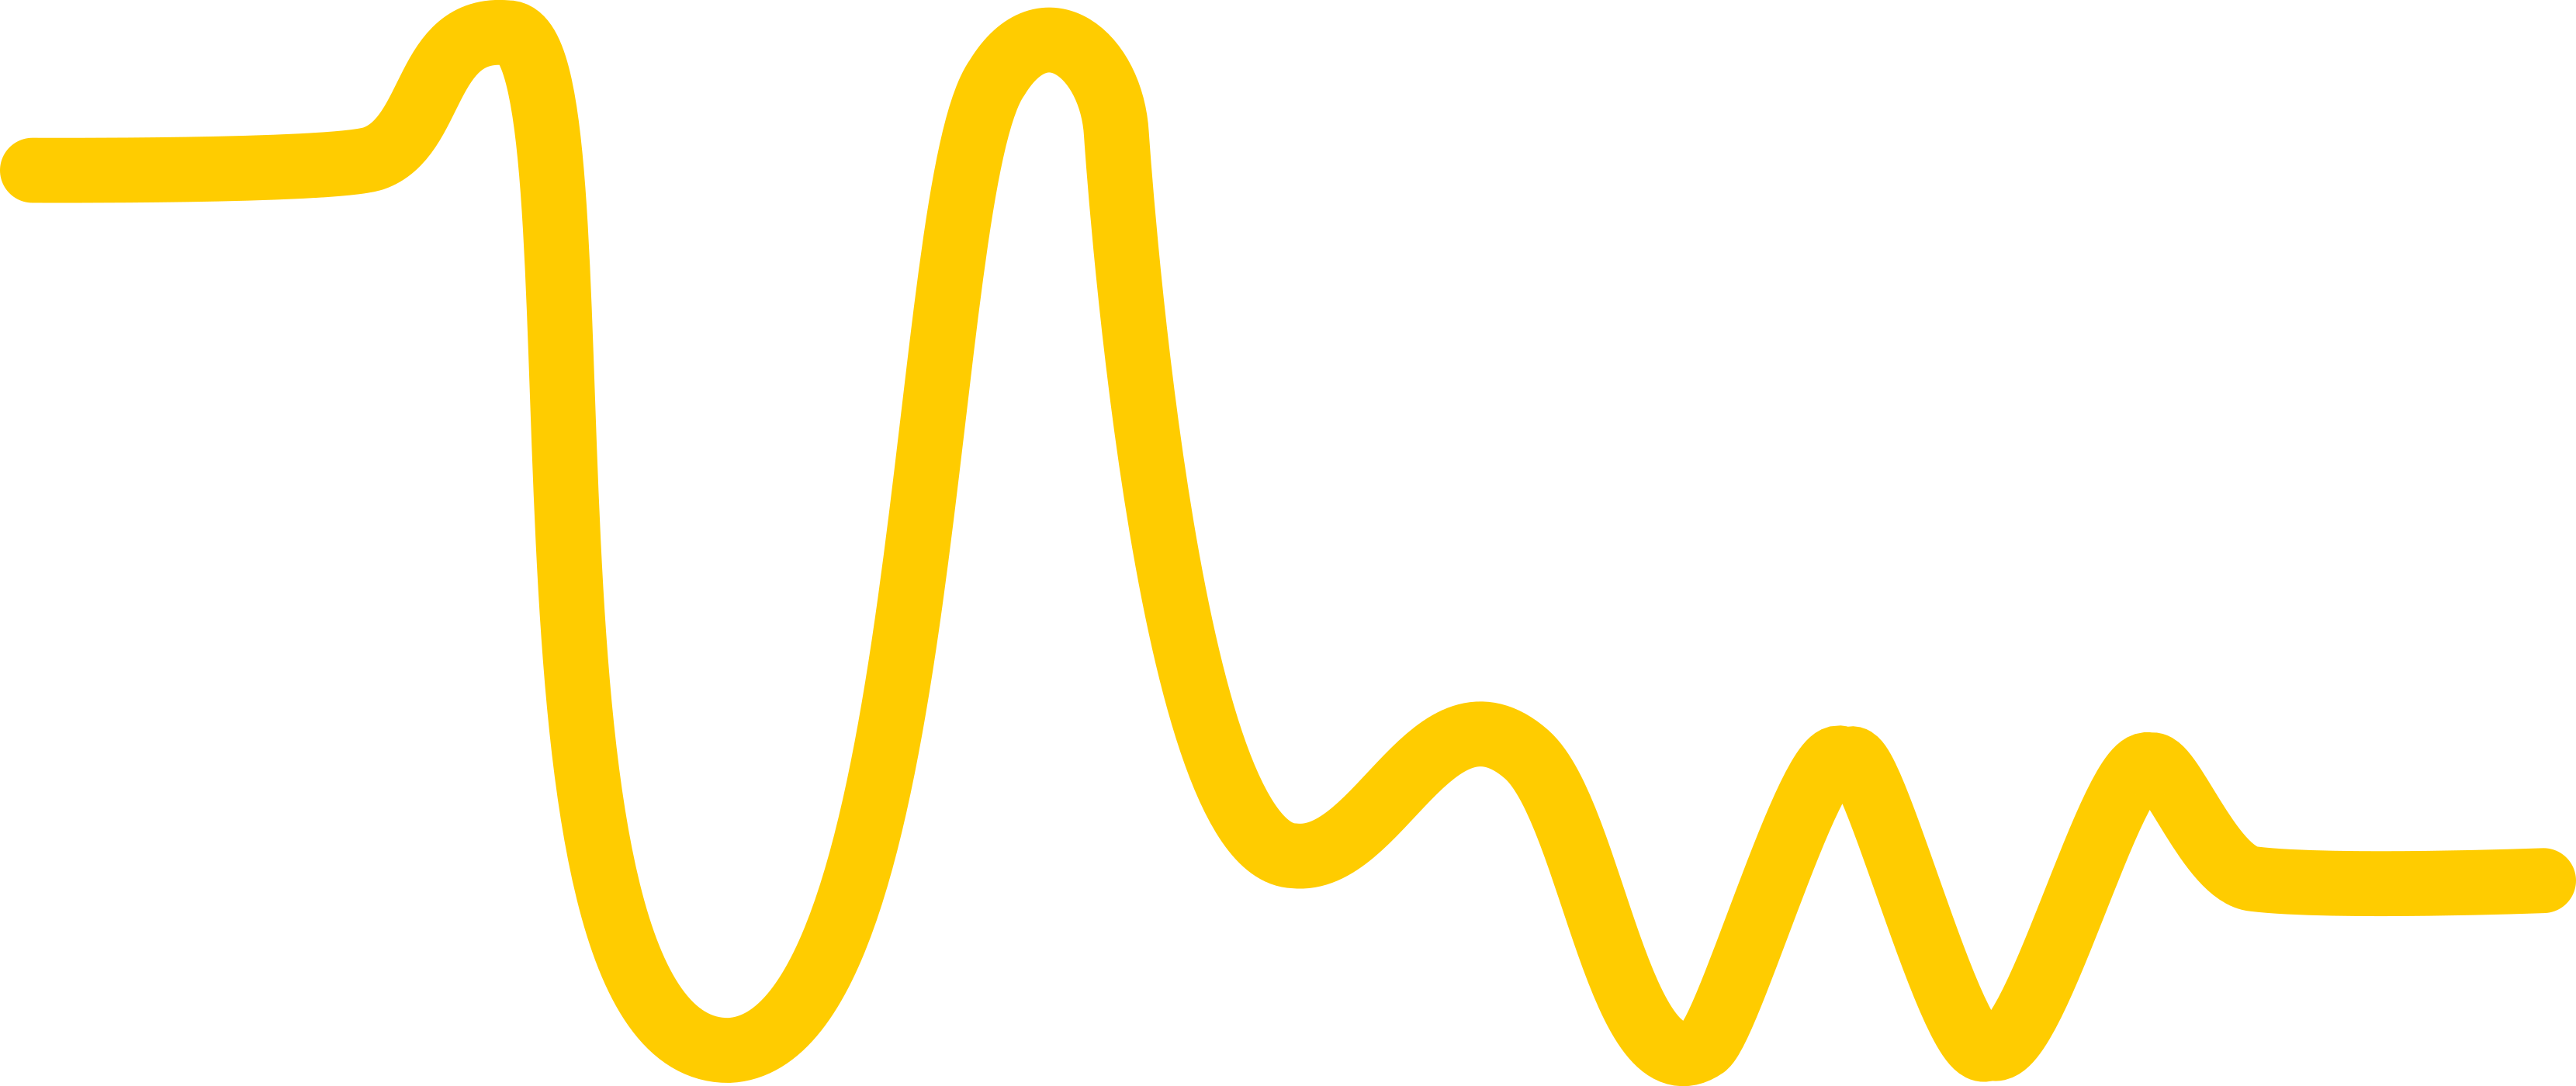
\includegraphics[width=0.20\paperwidth]{logo1.png}}
\author{\hspace{-40cm}\large Alexandre Avy, Hichem Khettab, Lou Marze, \\ \hspace{-40cm} Hamza Parnica, Guillaume Ung}
\date{Semester 5}

\begin{document}


\useblockstyle{bestblockstyle}

\maketitle[titletotopverticalspace=90mm,width = 0.5\paperwidth]

\block[titleoffsety=13cm,bodyoffsety=138mm,bodyverticalshift=10mm,titleinnersep=5mm,bodyinnersep=4mm,bodyoffsetx=80mm,bodywidthscale=.72,titlewidthscale=.4]{\textbf {Abstract}}{
\Large
% TODO: add phrase d'accroche on blind people et les besoins et la raison pour ce projet etc.
The goal of this semester project is to guide ,with sounds, a visually impaired person to follow a line. \\
The available tools are a Rasperry Pi and its camera.
For this goal, one needs to : \\
Detect the line from the camera's video \\
Process the line with the right technique \\
Find a way to communicate instructions to the user
}

\begin{columns}

\column{0.5}

\block{
\textbf{Video Processing}}{

\begin{center} \LARGE {Detecting the line}
\end{center}

\vspace{2mm}

\begin{center}
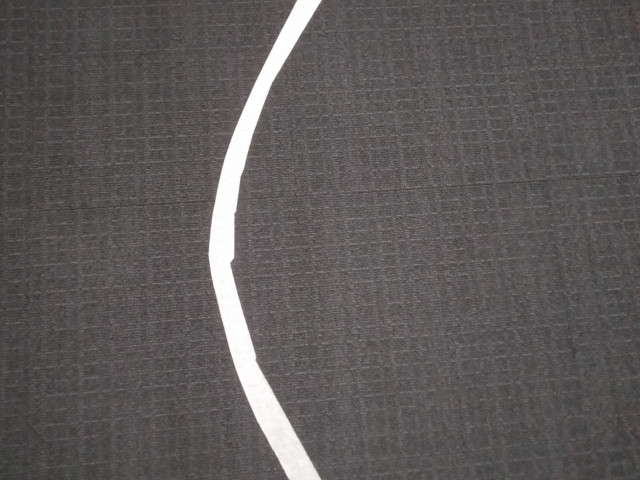
\includegraphics[height = 6cm, width = 6cm]{poster_images/reel3.jpg}
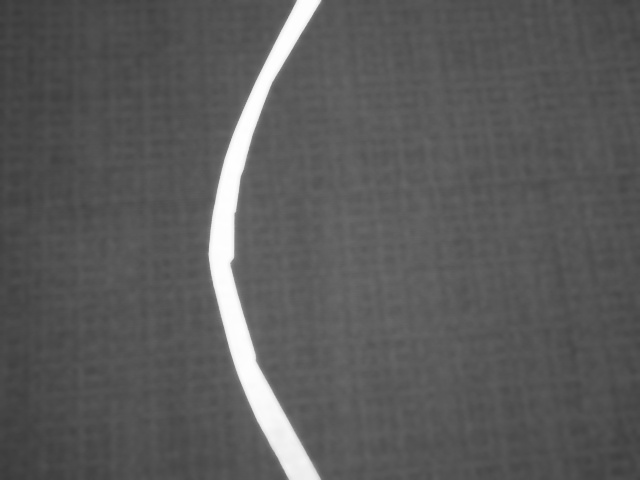
\includegraphics[height = 6cm, width = 6cm]{poster_images/gray.jpg}
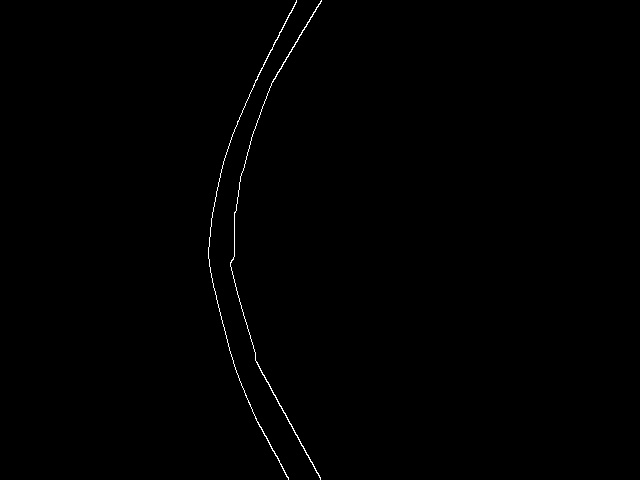
\includegraphics[height = 6cm, width = 6cm]{poster_images/canny_edge.jpg}
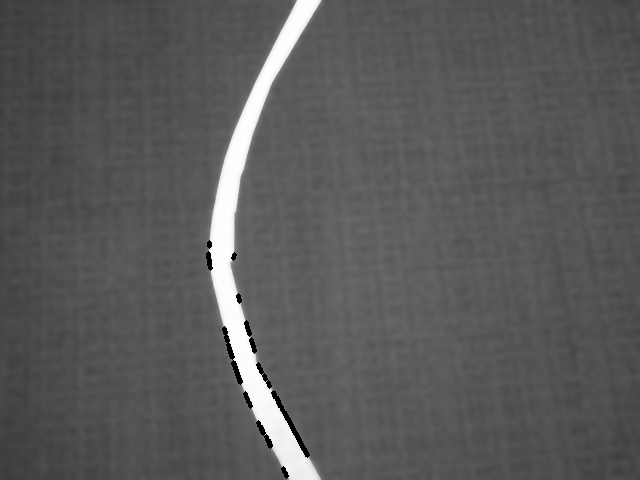
\includegraphics[height = 6cm, width = 6cm]{poster_images/houghlines_maybe.jpg}
\caption{\emph{Original image/Filtered image/Canny edge detection/Lines from Hough transform}}
% \centering\large Original image / Bilateral filter / Canny edge detection / Lines from Hough transform
\end{center}

Prior to detecting the line, the image is processed to optimize the detection quality through: \\
- Bilateral filtering \\
- Canny edge detection \\
Then Hough transform is applied to detect straight lines in the edges image.
 

% TODO: add caption, resize image and spacing
\vspace{2mm}

\begin{center} \LARGE {Computing the line direction}
\end{center}

\begin{center}
\frame{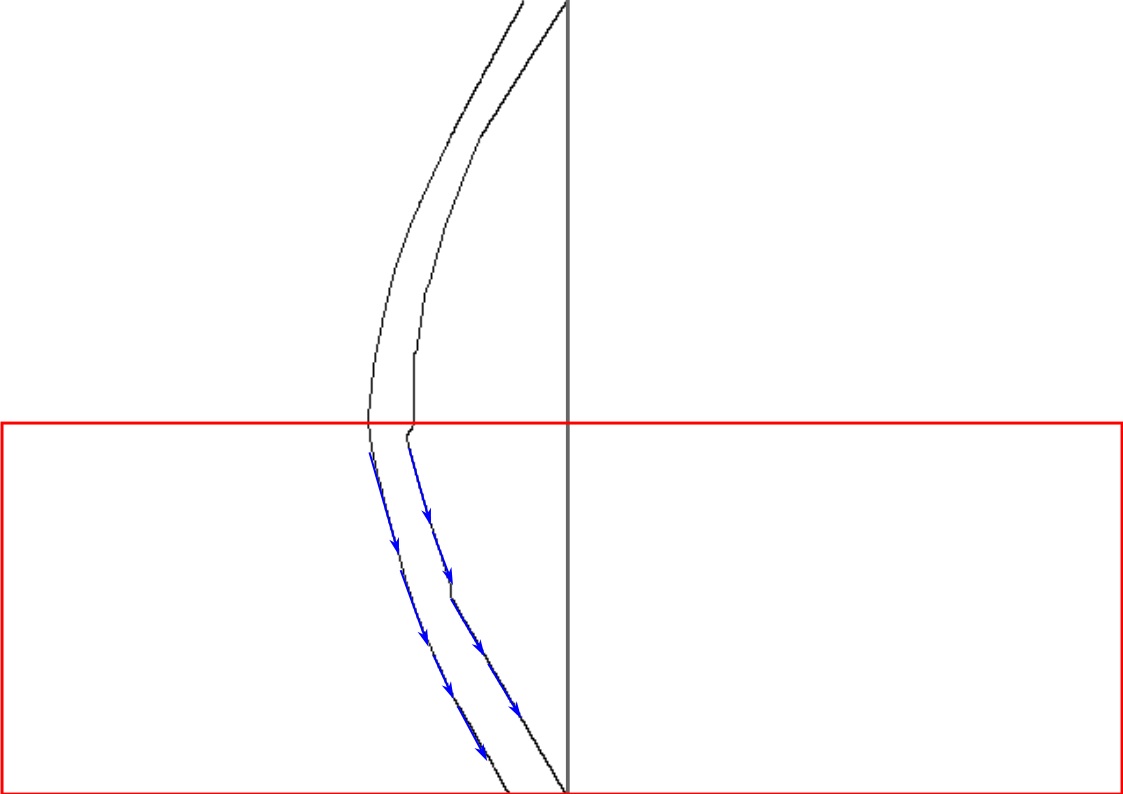
\includegraphics[width=0.40\linewidth,height = 7cm]{poster_images/angle_alpha1.png}}
\frame{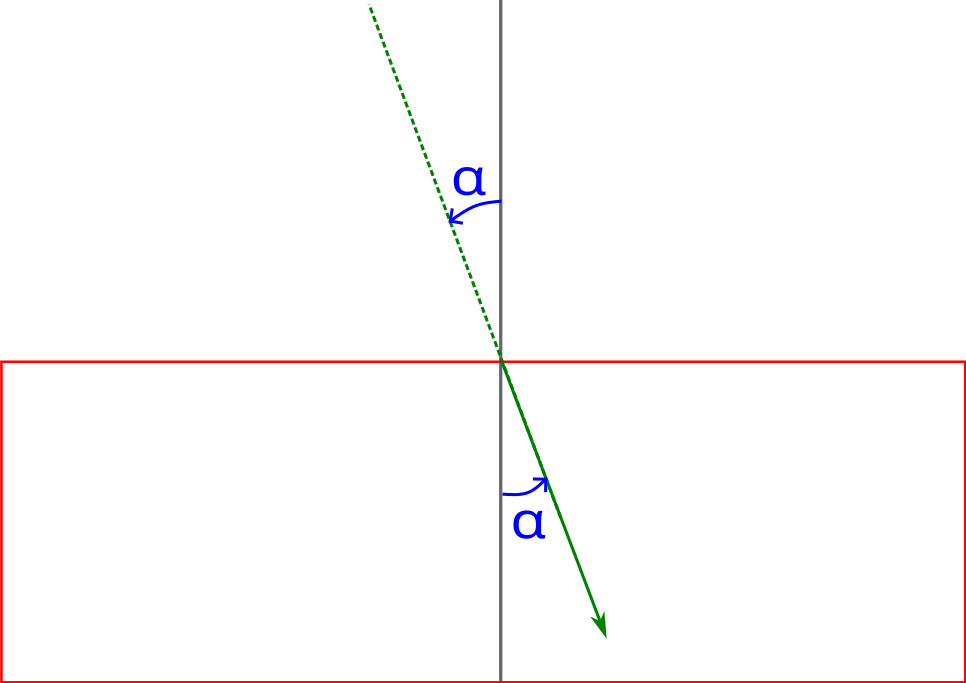
\includegraphics[width=0.40\linewidth,height =
7cm]{poster_images/angle_alpha.png}}
\\
\centering
\caption{\emph{Detected lines on bottom of the frame / Representation of the \(\alpha\) angle}}
\end{center}
The \(\alpha\) angle is defined as the average angle of the detected lines in the selected zone.
This selected zone is such that instructions are not given too early (which could misdirect the user)



% TODO: add caption, resize image and spacing

\begin{center} \LARGE {Taking the user position into account}
\end{center}

\begin{center}
\frame{\includegraphics[width=0.45\linewidth,height = 8cm]{distance_bas_barycentre.png}}
\frame{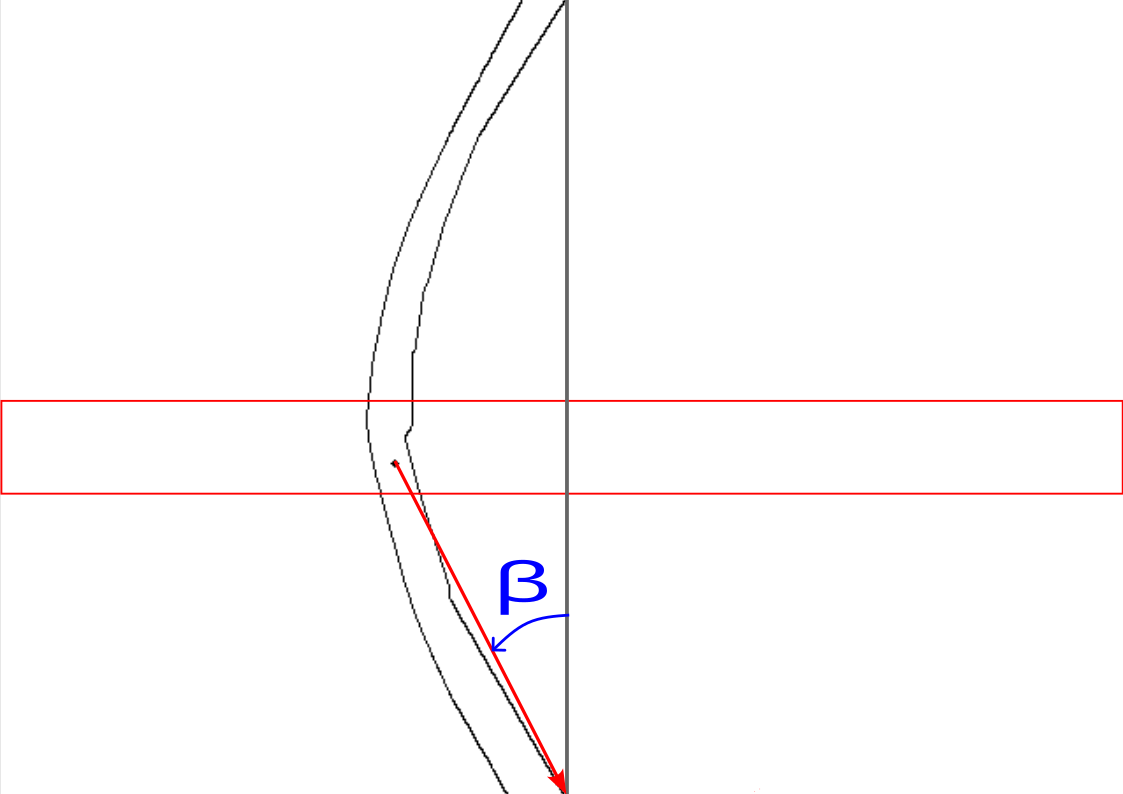
\includegraphics[width=0.45\linewidth,height = 8cm]{poster_images/angle_beta_barycentre_targetpoint.png}}
\\
\centering
\caption{\emph{Reprentation of the distance \(d\) and the \(\beta\) angle}}
\end{center}

Because the user could deviate from the line, we select the very bottom of the frame and look at the distance \(d\) between the barycentre of the line and the middle of the frame.
\\
If \(d\) is too important, the instruction to give is to get back on the line.\\
For this instruction, we define the \(\beta\) angle as represented :
\(\beta\) is the angle between the barycentre of the line in the target zone (in red) and the user.
This target zone is ahead of the user to plan for his movements and to optimize his travel time.





% \begin{center}
% \hspace{-0.7\linewidth}
% \includegraphics[width=0.2\linewidth]{poster_images/distance_bas_barycentre.png}
% \end{center}

% \begin{center}
% \hspace{0.2\linewidth}
% \vspace{90mm} \large dbneufnuizbnfueabfieja
% \end{center}
}

\column{0.5}


\block{Information processing}{

\begin{multicols}{2}

We want the final angle to reflect the distance of the user to the line, i.e.
we take more \(\alpha\) into account when \(d\) is small than \(\beta\), and
vice-versa. \\
Thus, we need a function \(f(d)\) that is close to 0 when \(d\) is small, and
close to 1 when \(d\) is big.


We choose

\[ f(d) = (1 - e^{\frac{-d}{\tau}}) \]

We choose \(\tau\) so that \(d_{95\%} = \frac{\text{width}}{2}\) (image
extremity), thus we have
\[ 3\tau = \frac{w}{2}, \quad \tau = \frac{w}{6} \]
It follows,
\[f(d) = 1 - e^{\frac{-6d}{w}}\]

Finally, we have

\[ \gamma = e^{\frac{-6d}{w}}\alpha + (1 - e^{\frac{-6d}{w}})\beta \]
\[ \gamma = \alpha + (1 - e^{\frac{-6d}{w}})(\beta - \alpha) \]


\columnbreak

\null \vfill

\begin{center}
\begin{tikzpicture}[scale=2]
\draw[>=stealth, ->] (0,0) -- (4,0);
\draw [>=stealth, ->] (0,0) -- (0,1.2);

\draw (4,0) node[right] {\(d\)};
\draw (3.8,1) node[right] {\(f(d)\)};

\draw (0,1) node[left] {\(1\)};
\draw [dashed] (0,1) -- (3.8,1);
\draw [dashed] (3,0) -- (3,0.95);
\draw (3,0) node[below] {\(d_{95\%}\)};
\draw [domain=0:3.8] plot (\x, {1-exp(-\x)});
\end{tikzpicture}
\end{center}

\vfill

\begin{center}
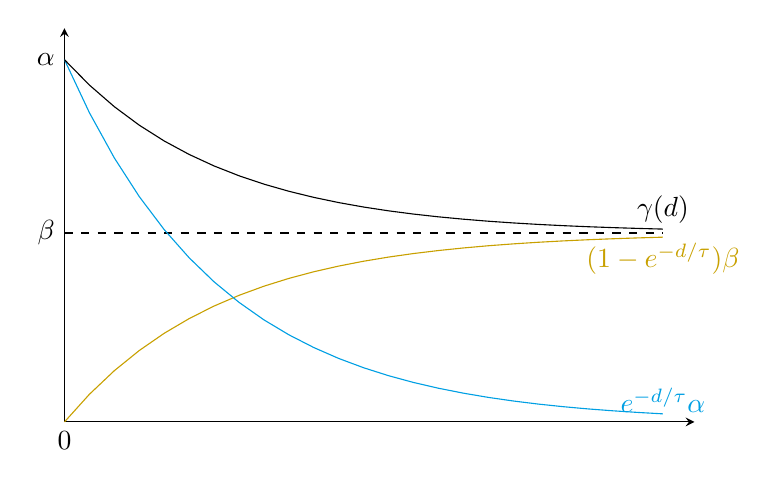
\begin{tikzpicture}[scale=2]
\draw[>=stealth, ->] (0,0) -- (4,0);
\draw [>=stealth, ->] (0,0) -- (0,2.5);
\draw (0,0) node[below] {\(0\)};

\draw [visuwalkorange, domain=0:3.8] plot (\x, {1.2*(1-exp(-\x))});
\draw [visuwalkorange] (3.8,1.2) node[below] {\((1-e^{-d/\tau})\beta\)};
\draw [dashed] (0,1.2) -- (3.8,1.2);
\draw (0,1.2) node[left] {\(\beta\)};

\draw [eurecomblue, domain=0:3.8] plot (\x, {2.3*(exp(-\x))});
\draw [eurecomblue] (3.8,0) node[above] {\(e^{-d/\tau}\alpha\)};
\draw (0,2.3) node[left] {\(\alpha\)};

\draw [domain=0:3.8] plot (\x, {2.3 - (1-exp(-\x))*1.1});
\draw (3.8,1.2) node[above] {\(\gamma(d)\)};

\end{tikzpicture}
\end{center}

\vfill \null

\end{multicols}

}

\block{\textbf{Sound Processing}}{

To guide the user , we decided to use stereo sound.
If the user has to go right, the sound will come from his right ear and vice versa.\\
The amplitude \emph{A} and frequency \emph{f} of the sound will vary depending on how sharp of a turn the user must make, following these formulas :
\[ A = 0.08\sqrt{|\gamma|} \]
\[ f = 3,9 |\gamma| + 230\]

}

\end{columns}
\block{\textbf{Conclusion}}{}


\end{document}
    
